% Anexo digital: importación del conteo físico desde la hoja de cálculo de la empresa.
% Se compila aparte (pdflatex ConteoFisico.tex) y se publica en tesis.pymetory.com/conteo-fisico.pdf.
% Pruebas medidas el 7-oct-2026 en local (PHPUnit, Playwright, axe-core). Datos de ejemplo inventados.
\documentclass[letterpaper,11pt]{article}
\usepackage[utf8]{inputenc}
\usepackage[T1]{fontenc}
\usepackage[spanish,es-noshorthands,es-tabla]{babel}
\usepackage{float}
\usepackage{graphicx}
\usepackage[margin=2.2cm]{geometry}
\usepackage{booktabs}
\usepackage{array}
\usepackage{tabularx}
\usepackage{enumitem}
\usepackage{xcolor}
\usepackage{url}
\usepackage[colorlinks=true,linkcolor=black,citecolor=black,urlcolor=blue!50!black]{hyperref}
\hypersetup{pdftitle={Pymetory — Importación del conteo físico},pdfauthor={Germán David Murillas Mondragón}}
\setlength{\parskip}{4pt}
\renewcommand{\arraystretch}{1.15}
\graphicspath{{Anexos/Imagenes/}}

\begin{document}

\begin{center}
{\LARGE\bfseries Pymetory}\\[4pt]
{\large Importación del conteo físico desde la hoja de cálculo de la empresa}\\[4pt]
Germán David Murillas Mondragón · Universidad del Valle, sede Tuluá · Anexo digital del trabajo de grado\\
{\small 7 de octubre de 2026}
\end{center}

\section{Propósito}

Para empezar a usar Pymetory, una PYME tiene que pasar al sistema lo que ya tiene en bodega, y después mantener el sistema igual a lo que hay físicamente. La panificadora del caso de estudio hace hoy esa tarea con una hoja de cálculo. El 6 de octubre de 2026 la administradora envió una foto de la hoja de inventario de materia prima y respondió seis preguntas sobre ella; autorizó usarla como evidencia, sin datos que identifiquen a la empresa. Sus respuestas definen el formato:

\begin{itemize}[nosep]
\item Las cantidades están en \textbf{kilos}.
\item Son el \textbf{conteo físico} de la bodega de materia prima al cierre del mes (``en existencia bodega de materia prima a Sept 30'').
\item Los números entre paréntesis del nombre, como en ``HARINA (50,38K)'', son las \textbf{presentaciones}: ``la harina viene por 50~k. Es el peso del bulto''.
\item Se crea una \textbf{pestaña nueva cada mes}.
\item Las diferencias se corrigen así: ``se hace una entrada o salida del sistema contable para iniciar mes con lo que existe en bodega''.
\end{itemize}

El módulo \textbf{Conteo físico} hace ese mismo procedimiento dentro de Pymetory: lee la hoja, la compara con el sistema y, cuando el administrador confirma, registra cada diferencia como un movimiento de ajuste del Kardex. No agrega reglas nuevas: aplica las cuatro del sistema (FEFO, Kardex inmutable, roles y datos tomados de la base de datos).

\section{Uso}

Está en el menú \textit{Gestión → Conteo físico} y solo lo ve el administrador; el servidor rechaza con 403 cualquier petición de un operario.

\begin{enumerate}[nosep]
\item Se elige el archivo (.xlsx o .csv, máximo 5~MB) y la unidad en que están las cantidades (kg por defecto).
\item \textit{Ver comparación} muestra, sin cambiar nada, cada insumo de la hoja con el insumo de Pymetory que le corresponde, la cantidad contada, la del sistema y la diferencia (Figura~\ref{fig:comparacion}).
\item Se revisan las filas: se puede cambiar la pestaña, las columnas detectadas o el insumo asignado a cada fila, y marcar o desmarcar cada ajuste.
\item \textit{Registrar ajustes en el Kardex} pide confirmación y crea los movimientos (Figuras~\ref{fig:resultado} y~\ref{fig:kardex}).
\end{enumerate}

\begin{figure}[H]
\centering
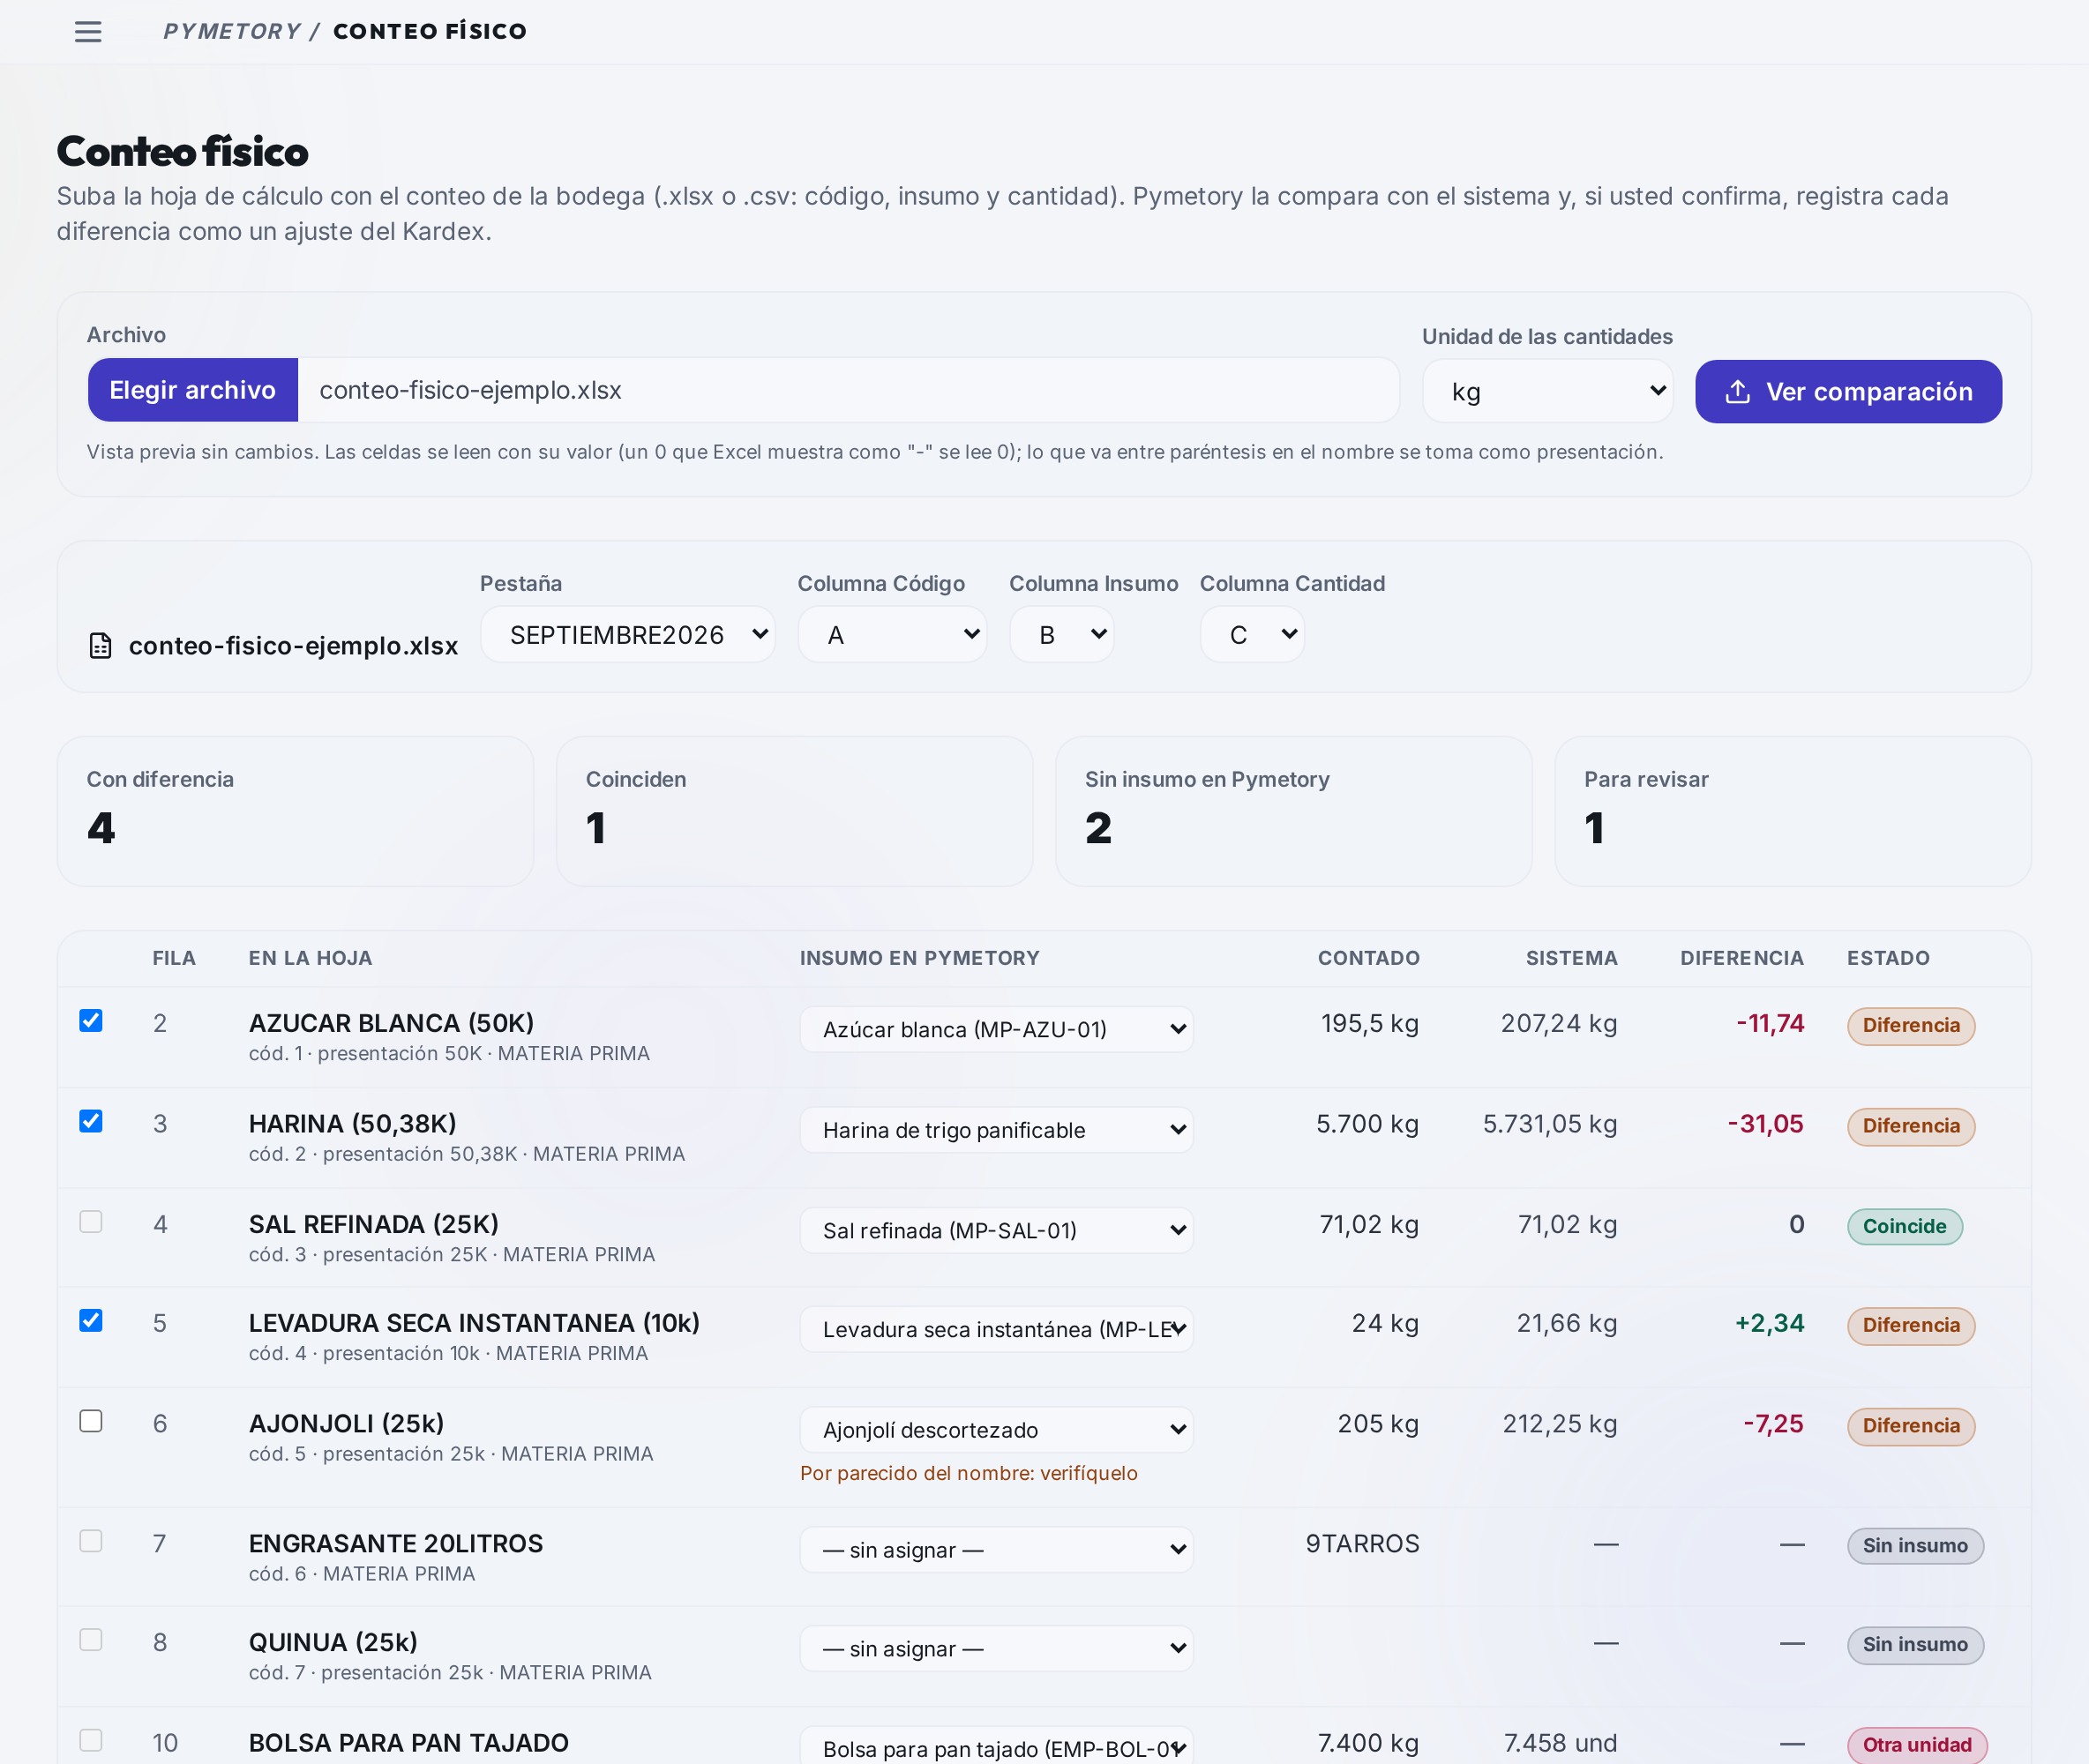
\includegraphics[width=\textwidth]{conteo-fisico.png}
\caption{Comparación de una hoja de ejemplo (datos inventados) con la base de demostración. ``HARINA'' se asignó a mano porque coincide con dos insumos.}
\label{fig:comparacion}
\end{figure}

\section{Funcionamiento}

\subsection{Lectura del archivo}

Un archivo .xlsx es un ZIP de archivos XML. El servidor de producción no tiene la extensión zip de PHP (por eso la exportación a Excel arma su propio ZIP), así que la lectura también se hace sin dependencias: la clase \texttt{XlsxLector} recorre el directorio central del ZIP, descomprime con \texttt{gzinflate} y lee el XML con SimpleXML. Se leen los \textbf{valores} de las celdas y no el texto formateado: un cero con formato contable que Excel muestra como ``-'' se lee como 0, y una celda vacía queda sin dato (no como cero). Por defecto se abre la pestaña que estaba activa al guardar el libro, que en una hoja mensual suele ser la del último mes. Contra archivos maliciosos, cada archivo interno descomprimido tiene un tope de 20~MB y el XML se lee sin resolver entidades externas.

\subsection{Interpretación de las filas}

La clase \texttt{ConciliacionConteo} detecta las columnas: la del insumo es la que tiene más letras; la de cantidad, la columna a su derecha con más números; la del código, la de su izquierda si tiene datos. Después clasifica cada fila:

\begin{itemize}[nosep]
\item Sin código ni cantidad (``MATERIA PRIMA'', ``INVENTARIO DE BOLSA''): título de sección; se muestra junto a los insumos que agrupa.
\item Lo que va entre paréntesis en el nombre se muestra como presentación, tal cual, sin interpretarlo.
\item Cantidades escritas como texto: se aceptan con separadores colombianos o ingleses (``1.204,60'', ``1,750.00''); una que no es número, como ``9TARROS'', queda para revisar.
\end{itemize}

\subsection{Emparejamiento con los insumos}

Cada fila se busca, en este orden, por código igual, por nombre igual (sin presentación, tildes ni mayúsculas) o por un nombre contenido en el otro, siempre que haya un único mejor candidato. Solo los dos primeros casos quedan marcados para aplicar; el tercero se muestra con el aviso ``por parecido del nombre: verifíquelo'' y sin marcar. Si hay empate (``HARINA'' con las dos harinas de la demostración) no se elige ninguno: se ofrecen sugerencias y el administrador decide. Un mismo insumo no puede quedar en dos filas.

Si la unidad de la hoja y la del insumo son distintas pero convertibles (kg y g, L y mL) se convierte; si no lo son (kilos contra unidades) la fila no se aplica.

\subsection{Registro de los ajustes}

Al confirmar, el servidor vuelve a calcular cada diferencia con el stock de ese momento, no con el de la vista previa, dentro de una transacción:

\begin{itemize}[nosep]
\item \textbf{Faltante:} sale de los lotes activos en orden \textbf{FEFO}, primero el que vence antes; un lote que queda en cero pasa a consumido.
\item \textbf{Sobrante:} entra al lote activo que vence más tarde.
\item \textbf{Insumo sin lotes activos:} no se aplica. Todo ingreso necesita un lote con su fecha de vencimiento para que FEFO funcione, así que el sistema no inventa uno: avisa que hay que registrarlo.
\end{itemize}

Cada movimiento queda con motivo \textit{ajuste}, el usuario que lo hizo y una descripción con la pestaña, el archivo, la cantidad contada y la del sistema. Nada se edita ni se borra (Kardex inmutable), y los ajustes no cuentan como consumo en Reabastecimiento, así que no alteran los pronósticos.

\begin{figure}[H]
\centering

\includegraphics[width=\textwidth]{conteo-fisico-resultado.png}
\caption{Resultado de registrar los ajustes de la Figura~\ref{fig:comparacion}.}
\label{fig:resultado}
\end{figure}

\begin{figure}[H]
\centering
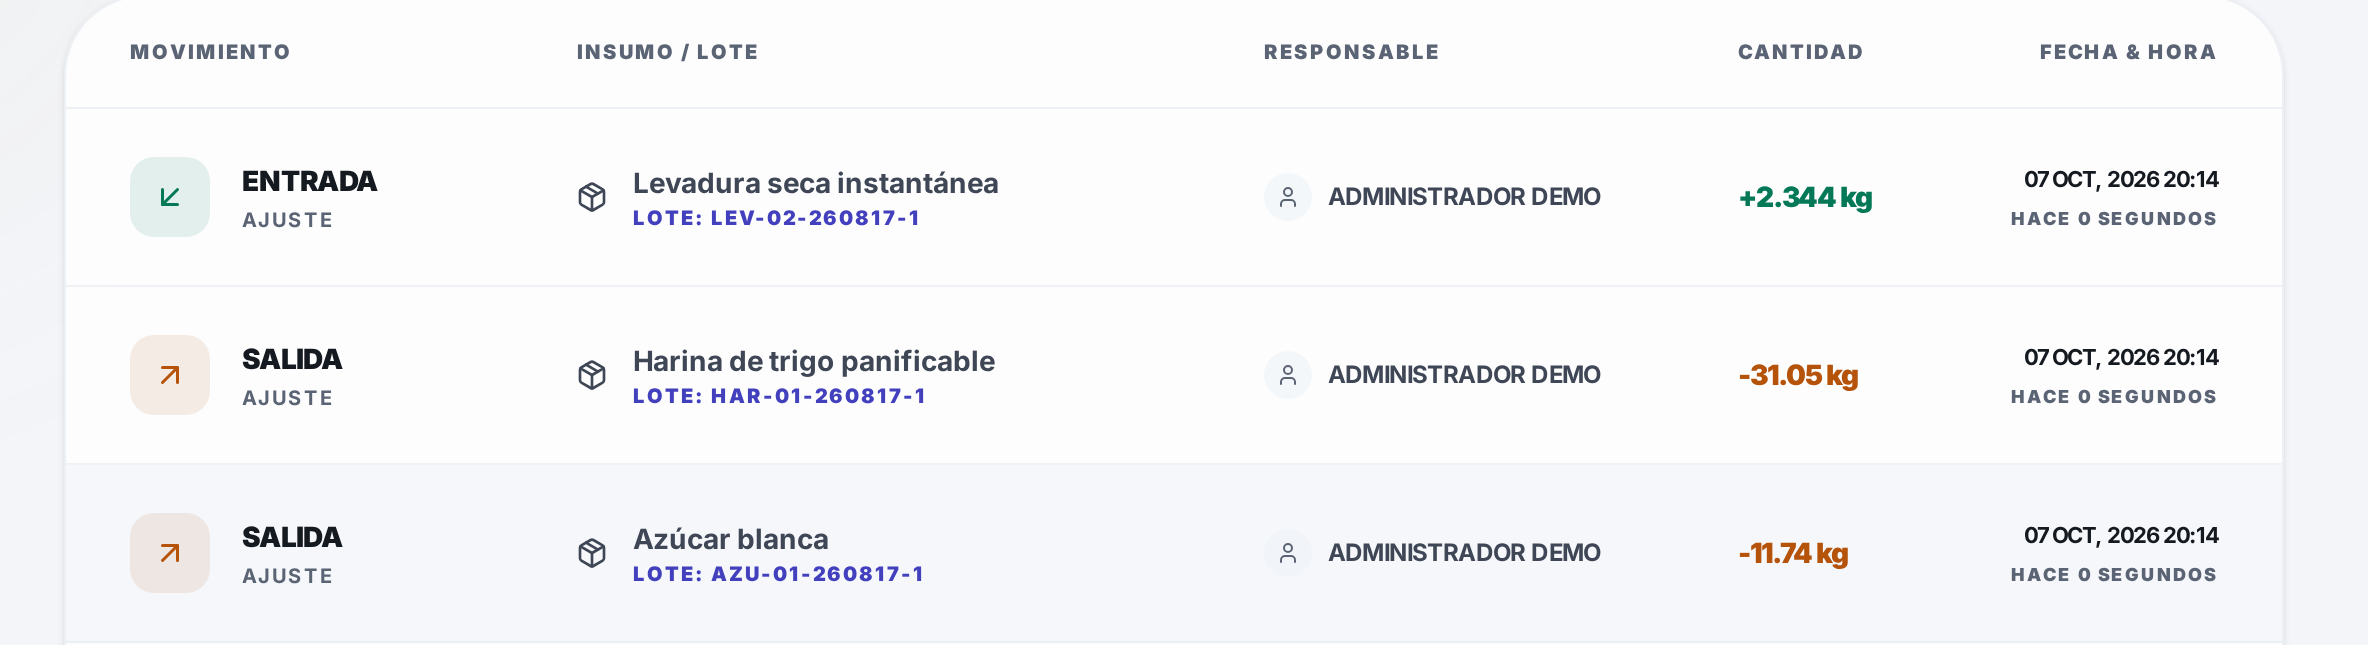
\includegraphics[width=\textwidth]{conteo-fisico-kardex.png}
\caption{Los tres movimientos de ajuste en el Kardex: dos faltantes (salidas) y un sobrante (entrada).}
\label{fig:kardex}
\end{figure}

\section{Pruebas}

Medidas el 7 de octubre de 2026 en el entorno local.

\begin{table}[H]
\centering
\begin{tabularx}{\textwidth}{lX}
\toprule
\textbf{Prueba} & \textbf{Qué verifica} \\
\midrule
PHPUnit (12 pruebas, 63 aserciones) & Lectura de un libro comprimido con textos compartidos y varias pestañas; lectura del .xlsx que exporta la propia aplicación; rechazo de archivos que no son .xlsx; números con separadores; detección de columnas, secciones, presentaciones y cantidades no numéricas; emparejamiento por código, nombre y parecido, y empates; conversión de kg a g; faltantes por FEFO y sobrantes en el lote más reciente; insumo sin lotes; la vista previa no modifica el inventario; CSV con punto y coma; un operario recibe 403; un insumo repetido se rechaza. \\
Playwright (2 pruebas) & Con el archivo de ejemplo: pestaña activa, estados de cada fila, asignación manual de un insumo y botón de registro habilitado; el módulo aparece en el menú del administrador. \\
axe-core, WCAG 2.1 AA & Vista con la comparación cargada en los seis temas, en escritorio y en celular: 0 incumplimientos. \\
\bottomrule
\end{tabularx}
\end{table}

Con estas, la suite PHPUnit completa pasa de las 178 reportadas en el Capítulo~11 del documento (medidas el 2 de octubre) a 190: 189 pasan y 1 se omite, con 701 aserciones.

\section{Limitaciones}

\begin{itemize}[nosep]
\item \textbf{Aún no se ha probado con el archivo real de la empresa}, solo con su foto y con hojas de ejemplo que imitan el formato. La prueba con el archivo real queda pendiente.
\item No crea insumos nuevos: las filas sin insumo en Pymetory se listan para registrarlos a mano con su categoría, bodega y lote.
\item Compara solo el stock activo; los lotes en cuarentena no se cuentan.
\item No lee el formato .xls antiguo (se debe guardar como .xlsx) ni fórmulas sin valor calculado.
\item Un número como ``1.750'' se lee como mil setecientos cincuenta, según la costumbre colombiana.
\item El emparejamiento por parecido puede equivocarse; por eso esas filas quedan sin marcar.
\end{itemize}

\section{Archivo de ejemplo}

En \url{https://tesis.pymetory.com/conteo-fisico-ejemplo.xlsx} hay una hoja con el mismo formato (dos pestañas mensuales, códigos, presentaciones entre paréntesis, secciones, una cantidad escrita como texto y una fila sin cantidad) y \textbf{datos inventados}, para probar el módulo en \url{https://app.pymetory.com}. No contiene datos de la empresa.

\section{Código}

\begin{itemize}[nosep]
\item \texttt{app/Support/XlsxLector.php}: lectura de .xlsx sin dependencias.
\item \texttt{app/Services/ConciliacionConteo.php}: interpretación, emparejamiento y registro de ajustes.
\item \texttt{app/Http/Controllers/ConciliacionController.php}: rutas \texttt{/conciliacion/vista-previa} y \texttt{/conciliacion/aplicar}.
\item \texttt{resources/js/components/Figma/FigmaConciliacion.tsx}: la vista.
\item \texttt{tests/Feature/ConciliacionConteoTest.php} y \texttt{tests/usabilidad/conteo-fisico.spec.cjs}: las pruebas.
\end{itemize}

Repositorio público: \url{https://github.com/germanmurillas/gestor-inventario-pymes-llm}.

\end{document}
